%%%%%%%%%%%%%%%%%%%%%%%%%%%%%%%%%%%%%%%%%%%%%%%%%%%%%%%%%%%%%%%%%%%%%%%%%%%%%%%
\chapter{Calor Específico de Sólidos} % Sem "Experiência 01" ou qualquer outro número
\label{Chap:CalorEspecifico}        % para poder trocar a ordem com facilidade
%%%%%%%%%%%%%%%%%%%%%%%%%%%%%%%%%%%%%%%%%%%%%%%%%%%%%%%%%%%%%%%%%%%%%%%%%%%%%%%

\begin{fullwidth}\it
Verificaremos o calor específico de alguns materiais, buscando comprovar experimentalmente as trocas energéticas envolvidas em transferências de calor. Veremos também a explicação para os fenômenos observados segundo a Primeira Lei da Termodinâmica. Utilizaremos os seguintes conceitos/técnicas de análise de dados: medidas, algarismos significativos, gráficos, software para elaboração de gráficos, erros de escala e propagados, equação geral para o erro propagado, regressão linear, linearização, erros dos coeficientes $A$ e $B$, e planílhas para cálculo dos coeficientes $A$ e $B$ com erros.
\end{fullwidth}

%%%%%%%%%%%%%%%%%%%%%%%%%%%%%%%%%%%%%%%%%%%%%%%%%%%%%%%%%%%%%%%%%%%%%%%%%%%%%%%
\section{Calor}
%%%%%%%%%%%%%%%%%%%%%%%%%%%%%%%%%%%%%%%%%%%%%%%%%%%%%%%%%%%%%%%%%%%%%%%%%%%%%%%

%Exp. acontece no início do estudo de termodinâmica, por isso precisamos explicar o qu é calor do ponto de vista de energia. Pra isso precisamos falar sobre trabalho e primeira lei da termodinâmica.

%Começar falando do calórico e da observação do Rumford ao perfurar os canhões

%Falar da Lei Zero da Termo.
%Falar sobre os processos de condução de calor e sobre a variação da energia interna e sua relação com a variação da temperatura/interpretação microscópica da temperatura.

%Falar sobre a determinação do equivalente mecânico para o calor

%O calor é armazenado como energia interna se $W=0$. Isso se reflete em uma mudanção na temperatura. No entanto, substâncias diferentes têm calore específicos diferentes. Por quê?
%Ver explicação do armazenamento de energia para um gás monoatômico e diatômico. Falar que o calor específico não é constante, que depende dos modos energéticos ativados. E que obviamente depende da fase do objeto (pq? deve ser pq mudam os modos de armazenamento de energia disponíveis)
%Ver sobre origens do calor específico dos sólidos.

%%%%%%%%%%%%%%%%%%%%%%%%%%%%%%%%%%%%%%%%%%
%\section{Determinação do Calor Específico}
%%%%%%%%%%%%%%%%%%%%%%%%%%%%%%%%%%%%%%%%%%

%%%%%%%%%%%%%%%%%%%%%%%%%%%%%%%%%%%%%%%%%%%%%%%%%%%%%%%%%%%%%%
\subsection{Determinação da Capacidade Térmica do Calorímetro}
%%%%%%%%%%%%%%%%%%%%%%%%%%%%%%%%%%%%%%%%%%%%%%%%%%%%%%%%%%%%%%

Para que possamos determinar o calor específico utilizando um calorímetro, devemos antes de tudo determinar qual é a quantidade de calor que será absorvida pelo próprio calorímetro. Se inicialmente temos o calorímetro e dentro dele uma massa de água $m_f$, sendo que ambos se encontram em equilíbrio térmico a uma temperatura $T^i$, ao adicionarmos uma massa $m_q$ de água quente, a uma temperatura $T_q$, obteremos uma temperatura final $T^f$. Analisando as trocas de calor, verificamos que
\begin{equation}
	Q^{\textrm{água quente}}_{\textrm{perdido}} + Q^{\textrm{água fria}}_{\textrm{ganho}} + Q^{\textrm{Calorímetro}}_{\textrm{ganho}} = 0.
\end{equation}
%
\begin{marginfigure}
	\centering
	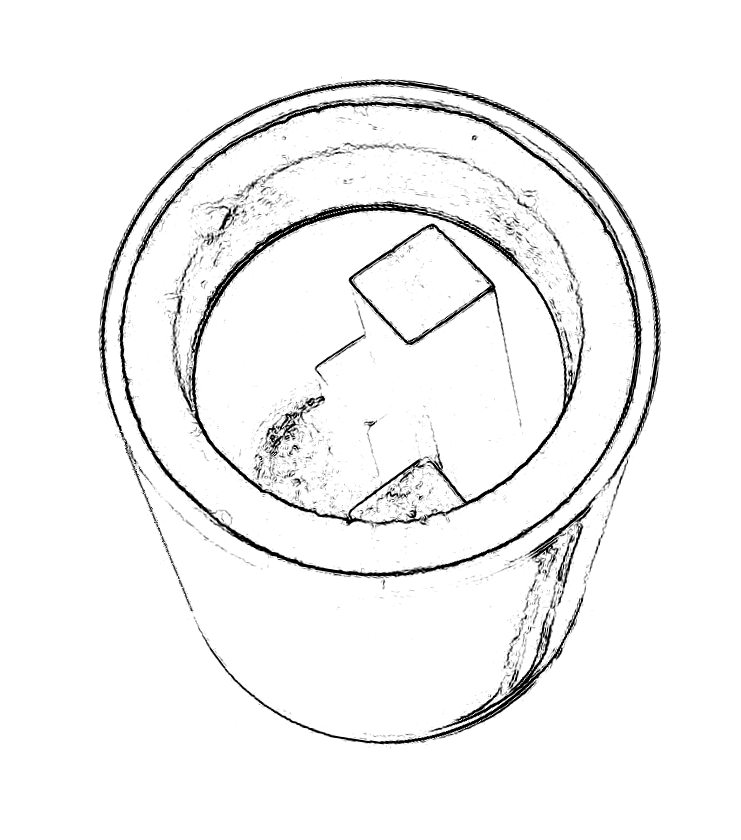
\includegraphics[width=0.8\textwidth]{Ilustrations/Calorimetro.png}
	\caption{Calorímetro aberto.}
\end{marginfigure}
Logo, se substituirmos $Q = mc\Delta T$ --~onde $c$ é o calor específico da água~-- para o calor ganho ou perdido pela água e $Q = C\Delta T$ --~onde $C$ é a capacidade térmica do calorímetro~--para o calor ganho pelo calorímetro, temos
\begin{equation}
	m_q c (T^f - T_q) + m_f c (T^f - T^i) + C(T^f - T^i) = 0,
\end{equation}
%
de onde obtemos
\begin{equation}
	C = -c\frac{m_q(T^f - T_q)+m_f(T^f - T^i)}{T^f - T^i}.
\end{equation}

%%%%%%%%%%%%%%%%%%%%%%%%%%%%%%%%%%%%%%%%%%%%%
\subsection{Determinação do Calor Específico}
%%%%%%%%%%%%%%%%%%%%%%%%%%%%%%%%%%%%%%%%%%%%%

\begin{margintable}
\begin{tabular}{ccc}
	\toprule
	Material & $\rm{J/kg\cdot\tcdegree C}$ & $\rm{cal/g\cdot\tcdegree C}$ \\
	\midrule
	Alumínio & 900 & \np{0,215} \\
	Cobre & 387 & \np{0,0924} \\
	Ferro & 448 & \np{0,107} \\
	Chumbo & 128 & \np{0,0305} \\
	Latão & 380 & \np{0,092} \\
	Água & 4186 & \np{1,00} \\
	\bottomrule
\end{tabular}
\caption{Calor específico para alguns materiais à temperatura de \np[\tcdegree C]{25}.% Tirei do Serway, talvez fosse melhor arranjar uma referência melhor, de alguém que medisse o treco e colocasse o erro pelo menos.
}
\end{margintable}
Para determinar o calor específico devemos tomar o calorímetro com uma massa $m$ de água fria, ambos em equilíbrio térmico a uma temperatura inicial $T^i$. Se tomarmos uma amostra aquecida a uma temperatura $T_q$ e o adicionarmos ao calorímetro, temos após o equilíbrio uma temperatura final $T^f$. Analisando as trocas de calor obtemos
\begin{equation}
	Q^{\textrm{Corpo}}_{\textrm{perdido}} + Q^{\textrm{água}}_{\textrm{ganho}} + Q^{\textrm{Calorímetro}}_{\textrm{ganho}} = 0
\end{equation}
%
Substituindo as expressões $Q = m c \Delta T$ para o ganho de calor pela água, $Q = m_a c_a \Delta T$ para o calor perdido pela amostra, e $Q = C\Delta T$ para o calor ganho pelo calorímetro, temos
\begin{equation}
	m_a c_a (T^f - T_q) + m c (T^f - T^i) + C (T^f-T^i) = 0.
\end{equation}
%
Obtemos então para o calor específico da amostra
\begin{equation}
	c_a = - \frac{mc(T^f-T^i) + C(T^f - T^i)}{m_a (T^f - T_q)}
\end{equation}

%%%%%%%%%%%%%%%%%%%%%%%%%%%%%%%%%%%%%%%%%%%%%%%%%%%%%%%%%%%%%%%%%%%%%%%%%%%%%%%
\section{Experimento}
%%%%%%%%%%%%%%%%%%%%%%%%%%%%%%%%%%%%%%%%%%%%%%%%%%%%%%%%%%%%%%%%%%%%%%%%%%%%%%%

%%%%%%%%%%%%%%%%%%%%%%
\subsection{Objetivos}
%%%%%%%%%%%%%%%%%%%%%%

\begin{itemize}
	\item Determinar experimentalmente o calor específicos de diferentes materiais sólidos;
	\item Observar a validade da Lei Zero da Termodinâmica;
	\item Observar a validade da Primeira Lei da Termodinâmica;
\end{itemize}

%%%%%%%%%%%%%%%%%%%%%%%%%%%%%%%%%%%%%%%%%%%%%%%%%%%%%%%%%%%%%%%%%%%%%%%%%%%%%%%
\section{Material Necessário}
%%%%%%%%%%%%%%%%%%%%%%%%%%%%%%%%%%%%%%%%%%%%%%%%%%%%%%%%%%%%%%%%%%%%%%%%%%%%%%%

\begin{itemize}
	\item Calorímetro;
	\item Termômetro de haste;
	\item Becker com água fria;
	\item Becker de vidro;
	\item Tripé, tela de amianto, lamparina a álcool e fósforos.
	\item Termômetro;
	\item Balança;
	\item Pinça;
	\item Corpos de diferentes materiais;
	\item Recipiente para descartar água.
\end{itemize}

\begin{figure}[!hbt]
	\centering
	\forcerectofloat
	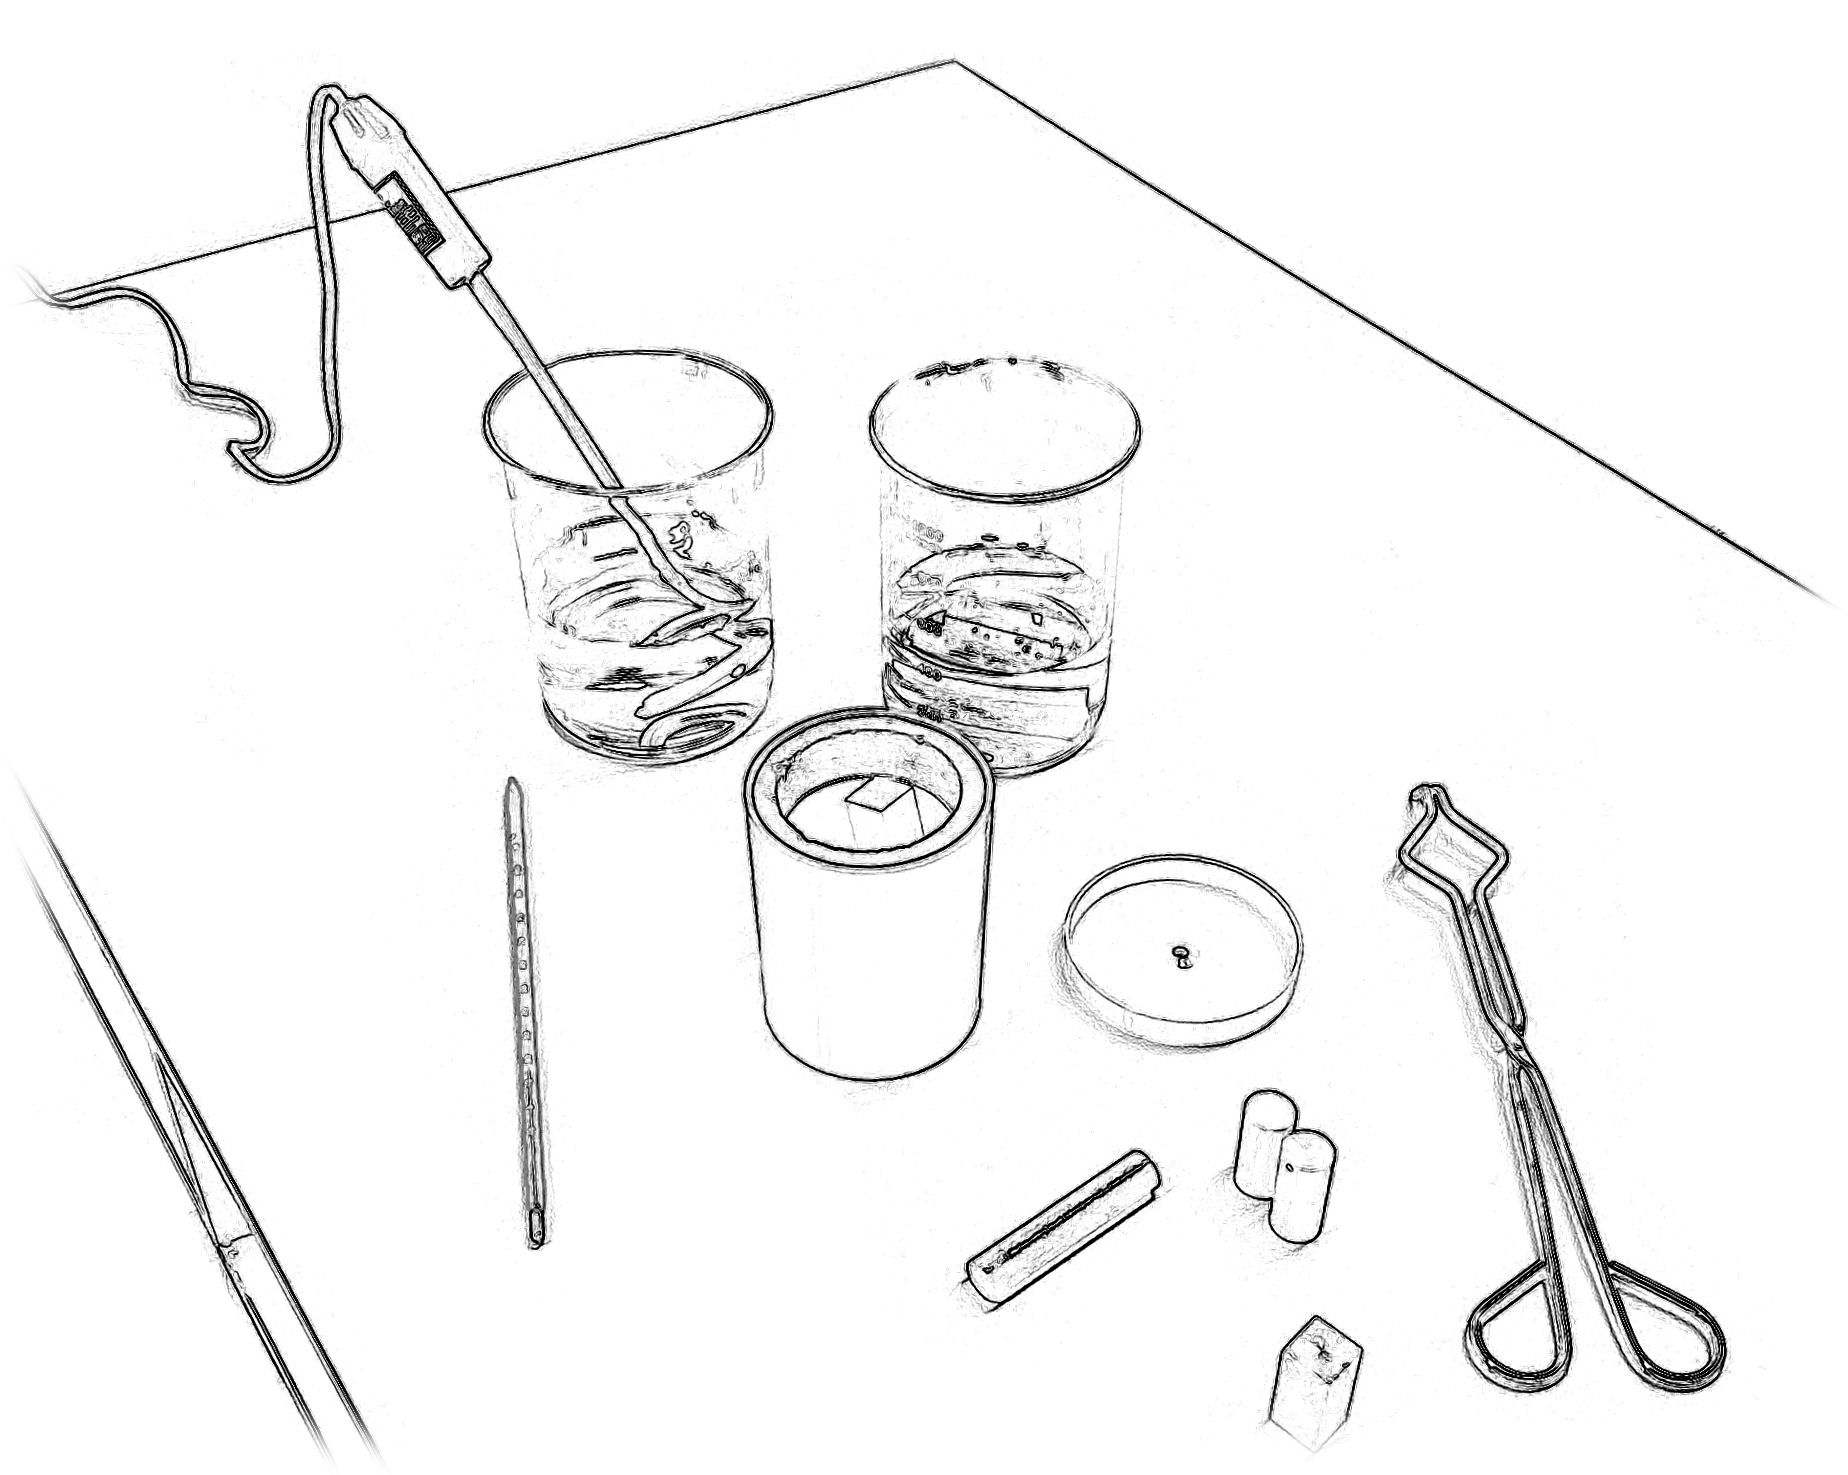
\includegraphics[width=0.7\textwidth]{Ilustrations/AparatoCalorEspecifico}
	\caption{Aparato para a verificação do calor específico de sólidos.}
\end{figure}

%%%%%%%%%%%%%%%%%%%%%%%%%%%%%%%%%%%%%%%%%%%%%%%%%%%%%%%%%%%%%%%%%%%%%%%%%%%%%%%
\section{Procedimento Experimental}
%%%%%%%%%%%%%%%%%%%%%%%%%%%%%%%%%%%%%%%%%%%%%%%%%%%%%%%%%%%%%%%%%%%%%%%%%%%%%%%

%%%%%%%%%%%%%%%%%%%%%
\subsection{Determinação da Capacidade Térmica do Calorímetro} % Se necessário
%%%%%%%%%%%%%%%%%%%%%
\begin{enumerate}
	\item Determine a massa do calorímetro com o auxílio da balança, anote o resultado na Tabela~\ref{Tab:CapacidadeTermica};
	\item Adicione água fria\footnote{Aqui ``água fria'' se refere a água a qualquer temperatura significativamente menor que a temperatura da água quente utilizada. Se a temperatura da água quente for de aproximadamente \np[\tcdegree C]{100,0}, por exemplo, para os nossos propósitos podemos considerar água à temperatura ambiente como fria.} ao calorímetro até que ela cubra aproximadamente um quarto da parte metálica interna;
	\item Verifique a massa do calorímetro com a água e anote na Tabela~\ref{Tab:CapacidadeTermica};
	\item Aguarde até que o sistema entre em equilíbrio térmico. Uma vez atingido o equilíbrio, com o auxílio do termômetro, determine a temperatura inicial do calorímetro. A partir de agora, mantenha o calorímetro sempre tampado;
	\item Verifique a temperatura da água quente disponível e anote na Tabela~\ref{Tab:CapacidadeTermica};
	\item Imediatamente após verificar a temperatura da água quente, adicione água quente ao calorímetro até cobrir aproximadamente a metade da cuba metálica interna. Aguarde o equilíbrio e verifique a temperatura do calorímetro, anotando na Tabela~\ref{Tab:CapacidadeTermica};
	\item Verifique a massa final do sistema;
	\item Descarte a água do calorímetro e repita o procedimento descrito acima mais duas vezes, anotando os dados na Tabela~\ref{Tab:CapacidadeTermica}
\end{enumerate}

%%%%%%%%%%%%%%%%%%%%%%%%%%%%%%%%%%%%%%%%%%%%%%%%%%%%%%%%
\subsection{Determinação do calor específico de sólidos}
%%%%%%%%%%%%%%%%%%%%%%%%%%%%%%%%%%%%%%%%%%%%%%%%%%%%%%%%

\begin{enumerate}
	\item Determine a massa do calorímetro com o auxílio da balança, anote o resultado na Tabela~\ref{Tab:CalorEspecifico};
	\item Adicione água fria ao calorímetro até que ela cubra aproximadamente um quarto da parte metálica interna;
	\item Verifique a massa do calorímetro com a água e anote na Tabela~\ref{Tab:CalorEspecifico};
	\item Aguarde até que o sistema entre em equilíbrio térmico. Uma vez atingido o equilíbrio, com o auxílio do termômetro, determine a temperatura inicial do calorímetro. A partir de agora, mantenha o calorímetro sempre tampado;
	\item Tome uma das amostras\footnote{Se houver mais que uma amostra do mesmo material disponível, tome mais que uma. Quanto maior for a massa, menor será o erro na determinação do calor específico.} e a submerja na água quente. Aguarde até que a amostra entre em equilíbrio térmico com a água. Verifique a temperatura da água e anote na Tabela~\ref{Tab:CalorEspecifico}.
	\item Retire a amostra do banho quente e o coloque rapidamente no calorímetro. Aguarde o equilíbrio térmico\footnote{Se as amostras forem metálicos, o equilíbrio será atingido rapidamente. Não aguarde um tempo muito longo pois nesse caso a energia térmica perdida pelo calorímetro para o ambiente será significativa.} e verifique a nova temperatura do calorímetro. Anote os resultados na Tabela~\ref{Tab:CalorEspecifico}.
	\item Retire a amostra do calorímetro, seque-o e verifique sua massa com o auxílio da balança.
	\item Repita o procedimento acima mais duas vezes para a mesma amostra. Após finalizar os procedimentos para a amostra em questão, repita todo o procedimento para cada um dos materiais disponíveis (três vezes).
\end{enumerate}

%%%%%%%%%%%%%%%%%%%%%%%%%%%%%%%%%%%%%%%%%%%%%%%%%%%%%%%%%%%%%%%%%%%%%%%%%%%%%%%
%%%%%%%%%%%%%%%%%%%%%%%%%%%%%%%%%%%%%%%%%%%%%%%%%%%%%%%%%%%%%%%%%%%%%%%%%%%%%%%
%%%%%%%%%%%%%%%%%%%%%%%%%%%%%%%%%%%%%%%%%%%%%%%%%%%%%%%%%%%%%%%%%%%%%%%%%%%%%%%
%%%%%%%%%%%%%%%%%%%%%%%%%%%%%%%%%%%%%%%%%%%%%%%%%%%%%%%%%%%%%%%%%%%%%%%%%%%%%%%
\cleardoublepage

\noindent{}{\huge\textit{Calor Específico de Sólidos}}

\vspace{15mm}

\begin{fullwidth}
\noindent{}\makebox[0.6\linewidth]{Turma:\enspace\hrulefill}\makebox[0.4\textwidth]{  Data:\enspace\hrulefill}
\vspace{5mm}

\noindent{}\makebox[0.6\linewidth]{Aluno(a):\enspace\hrulefill}\makebox[0.4\textwidth]{  Matrícula:\enspace\hrulefill}

\noindent{}\makebox[0.6\linewidth]{Aluno(a):\enspace\hrulefill}\makebox[0.4\textwidth]{  Matrícula:\enspace\hrulefill}

\noindent{}\makebox[0.6\linewidth]{Aluno(a):\enspace\hrulefill}\makebox[0.4\textwidth]{  Matrícula:\enspace\hrulefill}

\noindent{}\makebox[0.6\linewidth]{Aluno(a):\enspace\hrulefill}\makebox[0.4\textwidth]{  Matrícula:\enspace\hrulefill}

\noindent{}\makebox[0.6\linewidth]{Aluno(a):\enspace\hrulefill}\makebox[0.4\textwidth]{  Matrícula:\enspace\hrulefill}
\end{fullwidth}

\vspace{5mm}

%%%%%%%%%%%%%%%%%%%%%%%%%%%%%%%%%%%%%%%%%%%%%%%%%%%%%%%%%%%%%%%%%%%%%%%%%%%%%%%
\section{Questionário}
%%%%%%%%%%%%%%%%%%%%%%%%%%%%%%%%%%%%%%%%%%%%%%%%%%%%%%%%%%%%%%%%%%%%%%%%%%%%%%%

\begin{question}[type={exam}]{1}
Apresente os resultados de maneira clara e organizada. Mostre os cálculos requisitados de maneira clara e sucinta, evidenciando o raciocínio desenvolvido.
\end{question}

\begin{question}[type={exam}]{1}
Liste os equipamentos utilizados descrevendo o tipo do equipamento, sua resolução, e qual é o seu erro de escala.
\end{question}

\begin{question}[type={exam}]{2}
Preencha as tabelas com o número adequado de algarismos significativos, unidades, e erros de escala apropriados. 
\end{question}

\begin{question}[type={exam}]{2}
Calcule a capacidade térmica do calorímetro, juntamente com o erro propagado, para as três medidas realizadas. Obtenha o valor médio e o erro associado.
\end{question}

\begin{question}[type={exam}]{2}
Utilizando o resultado para a capacidade térmica do calorímetro e o erro associado a ela, calcule os calores específicos dos materiais, incluindo o erro propagado, para cada uma das três medidas de cada material. Obtenha o valor médio e o erro associado. Identifique o material com base no valor obtido para o calor específico e compare o resultado com os valores de referência calculando o erro percentual utilizando
\begin{equation}
	E_{\%} = \left|\frac{x-x_{\textrm{ref}}}{x_{\textrm{ref}}}\right| \times 100.
\end{equation}
\end{question}

\begin{question}[type={exam}]{2}
Através dos resultados obtidos nas questões anteriores, discuta quais objetivos foram atingidos com sucesso, justificando suas conclusões. Se algum objetivo não foi atingido, discuta quais são os possíveis motivos do fracasso e que providências podem ser tomadas para que eles sejam alcançados.
\end{question}

\vfill
%%%%%%%%%%%%%%%%%%%%%%%%%%%%%%%%%%%%%%%%%%%%%%%%%%%%%%%%%%%%%%%%%%%%%%%%%%%%%%%
\pagebreak
\section{Tabelas}
%%%%%%%%%%%%%%%%%%%%%%%%%%%%%%%%%%%%%%%%%%%%%%%%%%%%%%%%%%%%%%%%%%%%%%%%%%%%%%%

\begin{table*}[!ht]
\centering
	\begin{tabular}{lp{22mm}p{22mm}p{22mm}lp{22mm}p{22mm}p{22mm}l}
		\toprule
		&\multicolumn{6}{l}{\textbf{Determinação da Capacidade Térmica do calorímetro}}\\
		\cmidrule{2-8}
		&\multicolumn{3}{c}{Massas} & & \multicolumn{3}{c}{Temperaturas}& \\
		\cmidrule{2-4}\cmidrule{6-8}
		& $m^{\rm{Cal}}$ & $m^{\textrm{Cal + água}}_{\rm{fria}}$ & $m^{\textrm{Cal + água}}_{\textrm{fria + quente}}$ & & $T^{\rm{Cal}}_{i}$ & $T^{\textrm{água}}_{\textrm{quente}}$ & $T^{\rm{Cal}}_{f}$ & \\
		\cmidrule{2-4}\cmidrule{6-8}
		& \cellcolor[gray]{0.95} & \cellcolor[gray]{0.97} & \cellcolor[gray]{0.95} & & \cellcolor[gray]{0.95} & \cellcolor[gray]{0.97} & \cellcolor[gray]{0.95} & \\
		& \cellcolor[gray]{0.89} & \cellcolor[gray]{0.92} & \cellcolor[gray]{0.89} & & \cellcolor[gray]{0.89} & \cellcolor[gray]{0.92} & \cellcolor[gray]{0.89} & \\
		& \cellcolor[gray]{0.95} & \cellcolor[gray]{0.97} & \cellcolor[gray]{0.95} & & \cellcolor[gray]{0.95} & \cellcolor[gray]{0.97} & \cellcolor[gray]{0.95} & \\
		\cmidrule{2-8}
		\bottomrule
	\end{tabular}
	\caption[][1cm]{Dados para o cálculo da capacidade térmica do calorímetro.}
	\label{Tab:CapacidadeTermica}
\end{table*}

\begin{table*}[!ht]
\centering
\forcerectofloat
	\begin{tabular}{lp{22mm}p{22mm}p{22mm}lp{22mm}p{22mm}p{22mm}l}
		\toprule
\multicolumn{6}{l}{\textbf{Determinação do Calor Específico}}\\
\\
		&\multicolumn{6}{l}{\textbf{Corpo 1}}\\
		\cmidrule{2-8}
		&\multicolumn{3}{c}{Massas} & & \multicolumn{3}{c}{Temperaturas}& \\
		\cmidrule{2-4}\cmidrule{6-8}
		& $m^{\rm{Cal}}$ & $m^{\textrm{Cal + água}}_{\rm{fria}}$ & $m^{\textrm{amostra}}$ & & $T^{\rm{Cal}}_{i}$ & $T^{\textrm{água}}_{\textrm{quente}}$ & $T^{\rm{Cal}}_{f}$ & \\
		\cmidrule{2-4}\cmidrule{6-8}
		& \cellcolor[gray]{0.95} & \cellcolor[gray]{0.97} & \cellcolor[gray]{0.95} & & \cellcolor[gray]{0.95} & \cellcolor[gray]{0.97} & \cellcolor[gray]{0.95} & \\
		& \cellcolor[gray]{0.89} & \cellcolor[gray]{0.92} & \cellcolor[gray]{0.89} & & \cellcolor[gray]{0.89} & \cellcolor[gray]{0.92} & \cellcolor[gray]{0.89} & \\
		& \cellcolor[gray]{0.95} & \cellcolor[gray]{0.97} & \cellcolor[gray]{0.95} & & \cellcolor[gray]{0.95} & \cellcolor[gray]{0.97} & \cellcolor[gray]{0.95} & \\
		\cmidrule{2-8}
\\
		&\multicolumn{6}{l}{\textbf{Corpo 2}}\\
		\cmidrule{2-8}
		&\multicolumn{3}{c}{Massas} & & \multicolumn{3}{c}{Temperaturas}& \\
		\cmidrule{2-4}\cmidrule{6-8}
		& $m^{\rm{Cal}}$ & $m^{\textrm{Cal + água}}_{\rm{fria}}$ & $m^{\textrm{amostra}}$ & & $T^{\rm{Cal}}_{i}$ & $T^{\textrm{água}}_{\textrm{quente}}$ & $T^{\rm{Cal}}_{f}$ & \\
		\cmidrule{2-4}\cmidrule{6-8}
		& \cellcolor[gray]{0.95} & \cellcolor[gray]{0.97} & \cellcolor[gray]{0.95} & & \cellcolor[gray]{0.95} & \cellcolor[gray]{0.97} & \cellcolor[gray]{0.95} & \\
		& \cellcolor[gray]{0.89} & \cellcolor[gray]{0.92} & \cellcolor[gray]{0.89} & & \cellcolor[gray]{0.89} & \cellcolor[gray]{0.92} & \cellcolor[gray]{0.89} & \\
		& \cellcolor[gray]{0.95} & \cellcolor[gray]{0.97} & \cellcolor[gray]{0.95} & & \cellcolor[gray]{0.95} & \cellcolor[gray]{0.97} & \cellcolor[gray]{0.95} & \\
		\cmidrule{2-8}
\\
		&\multicolumn{6}{l}{\textbf{Corpo 3}}\\
		\cmidrule{2-8}
		&\multicolumn{3}{c}{Massas} & & \multicolumn{3}{c}{Temperaturas}& \\
		\cmidrule{2-4}\cmidrule{6-8}
		& $m^{\rm{Cal}}$ & $m^{\textrm{Cal + água}}_{\rm{fria}}$ & $m^{\textrm{amostra}}$ & & $T^{\rm{Cal}}_{i}$ & $T^{\textrm{água}}_{\textrm{quente}}$ & $T^{\rm{Cal}}_{f}$ & \\
		\cmidrule{2-4}\cmidrule{6-8}
		& \cellcolor[gray]{0.95} & \cellcolor[gray]{0.97} & \cellcolor[gray]{0.95} & & \cellcolor[gray]{0.95} & \cellcolor[gray]{0.97} & \cellcolor[gray]{0.95} & \\
		& \cellcolor[gray]{0.89} & \cellcolor[gray]{0.92} & \cellcolor[gray]{0.89} & & \cellcolor[gray]{0.89} & \cellcolor[gray]{0.92} & \cellcolor[gray]{0.89} & \\
		& \cellcolor[gray]{0.95} & \cellcolor[gray]{0.97} & \cellcolor[gray]{0.95} & & \cellcolor[gray]{0.95} & \cellcolor[gray]{0.97} & \cellcolor[gray]{0.95} & \\
		\cmidrule{2-8}
\\
		&\multicolumn{6}{l}{\textbf{Corpo 4}}\\
		\cmidrule{2-8}
		&\multicolumn{3}{c}{Massas} & & \multicolumn{3}{c}{Temperaturas}& \\
		\cmidrule{2-4}\cmidrule{6-8}
		& $m^{\rm{Cal}}$ & $m^{\textrm{Cal + água}}_{\rm{fria}}$ & $m^{\textrm{amostra}}$ & & $T^{\rm{Cal}}_{i}$ & $T^{\textrm{água}}_{\textrm{quente}}$ & $T^{\rm{Cal}}_{f}$ & \\
		\cmidrule{2-4}\cmidrule{6-8}
		& \cellcolor[gray]{0.95} & \cellcolor[gray]{0.97} & \cellcolor[gray]{0.95} & & \cellcolor[gray]{0.95} & \cellcolor[gray]{0.97} & \cellcolor[gray]{0.95} & \\
		& \cellcolor[gray]{0.89} & \cellcolor[gray]{0.92} & \cellcolor[gray]{0.89} & & \cellcolor[gray]{0.89} & \cellcolor[gray]{0.92} & \cellcolor[gray]{0.89} & \\
		& \cellcolor[gray]{0.95} & \cellcolor[gray]{0.97} & \cellcolor[gray]{0.95} & & \cellcolor[gray]{0.95} & \cellcolor[gray]{0.97} & \cellcolor[gray]{0.95} & \\
		\cmidrule{2-8}
		\bottomrule
	\end{tabular}
	\caption[][1cm]{Dados para o cálculo do calor específico de diferentes materiais.}
	\label{Tab:CalorEspecifico}
\end{table*}

\vfill


